\documentclass[a4paper,10pt]{article}
\usepackage[utf8]{inputenc}
\usepackage[spanish]{babel}
\usepackage[affil-it]{authblk}
\usepackage{enumerate}
\usepackage{graphicx}
\usepackage{hyperref}
\usepackage{amsmath}
\usepackage{amssymb}
\usepackage{cancel}
\usepackage[usenames, dvipsnames]{color}
\usepackage{tikz}
\usepackage{multimedia}
\usepackage{subcaption} %Multiple images
\usepackage{multicol} % Multiple columns
\usepackage{float}
\usepackage{cleveref}
\usepackage[margin=1.4in]{geometry}
\usepackage[labelfont=bf]{caption}
\usetikzlibrary{calc}
\numberwithin{equation}{section}

%Columns separation
\setlength{\columnsep}{1cm}

%Indentation
\setlength{\parindent}{0ex}

%Multiple References

\usepackage{xparse}
\ExplSyntaxOn
\NewDocumentCommand{\mref}{m}{\quinn_mref:n {#1}}
\seq_new:N \l_quinn_mref_seq
\cs_new:Npn \quinn_mref:n #1
 {
  \seq_set_split:Nnn \l_quinn_mref_seq { , } { #1 }
  \seq_pop_right:NN \l_quinn_mref_seq \l_tmpa_tl
  ( % print the left parenthesis
  \seq_map_inline:Nn \l_quinn_mref_seq
    { \ref{##1},\nobreakspace } % print the first references
  \exp_args:NV \ref \l_tmpa_tl 
  ) 
 }
\ExplSyntaxOff


%Boxes

\newcommand*{\boxcolor}{blue}
\makeatletter
\renewcommand{\boxed}[1]{\textcolor{\boxcolor}{%
\tikz[baseline={([yshift=-1ex]current bounding box.center)}] \node [rectangle, minimum width=1ex,rounded corners,draw] {\normalcolor\m@th$\displaystyle#1$};}}
 \makeatother

%Constantes
\newcommand{\euler}{\mathrm{e}}
\newcommand{\im}{i}

%Lemas, teoremas, definiciones y pruebas
\newcommand{\definicion}{\textbf{Definición: }}
\newcommand{\lema}{\textbf{Lema: }}
\newcommand{\teorema}{\textbf{Teorema: }}
\newcommand{\prueba}{\textbf{Prueba: }}


%opening
\title{Mecánica Clásica Tarea \# 5}
\author{Favio Vázquez\thanks{Correo: favio.vazquezp@gmail.com}}\affil{Instituto de Ciencias Nucleares. Universidad Nacional Autónoma de México.}
\date{}

\begin{document}

\makeatletter
\def\@maketitle{%
  \newpage
  \null
  \vskip 2em%
  \begin{center}%
  \let \footnote \thanks
    {\Large\bfseries \@title \par}%
    \vskip 1.5em%
    {\normalsize
      \lineskip .5em%
      \begin{tabular}[t]{c}%
        \@author
      \end{tabular}\par}%
    \vskip 1em%
    {\normalsize \@date}%
  \end{center}%
  \par
  \vskip 1.5em}
\makeatother

\maketitle

\section{Problema 1}

Dos partículas, una de masa $m_1$ y otra de masa $m_2$, interaccionan gravitacionalmente 
en el espacio tridimensional. En adición a su interacción mutua se encuentran en un campo 
de fuerzas externo que les produce una aceleración constante $\mathbf{a}$ en cierta 
dirección también constante. En un sistema de coordenadas generalizadas conveniente para este 
sistema, encuentre la función lagrangiana y las ecuaciones de movimiento.

\vspace{.3cm}

\underline{Solución:} \vspace{.3cm}

\section{Problema 2}

Demuestre que si la energía cinética de un sistema mecánico se puede expresar como

$$
T = \sum_i f_i(q^i)(\dot{q}^i)^2,
$$

y la energía potencial como

$$
V = \sum_i V_i(q^i),
$$

entonces podemos reducir a cuadraturas las ecuaciones de movimiento.

\vspace{.3cm}

\underline{Solución:} \vspace{.3cm}

Tenemos las siguientes expresiones para la energía cinética y potencial del sistema,

\begin{equation}
 T = \sum_i f_i(q^i)(\dot{q}^i)^2,
 \label{eq:2cinetica1}
\end{equation}

\begin{equation}
 V = \sum_i V_i(q^i).
 \label{eq:2potencial1}
\end{equation}

Y podemos escribir la lagrangiana $L = T - V$ del sistema como,

\begin{equation}
 L = \sum_i \left[ f_i(q^i)(\dot{q}^i)^2 - V_i(q^i)\right] = \sum_i L_i,
\end{equation}

donde

\begin{equation}
 L_i = f_i(q^i)(\dot{q}^i)^2 - V_i(q^i).
\end{equation}

Por otra parte las ecuaciones de Lagrange nos dicen que,

\begin{equation}
 \frac{d}{dt} \frac{\partial L}{\partial \dot{q}^i} = \frac{\partial L}{\partial q^i},
\end{equation}

pero debido a que $L_i$ solo depende de $\dot{q}^i$ y $q^i$, entonces

\begin{equation}
 \frac{d}{dt} \frac{\partial L_i}{\partial \dot{q}^i} = \frac{\partial L_i}{\partial q^i}. 
 \label{eq:3ecdeLagrange1}
\end{equation}

Y vemos entonces que las ecuaciones se separan y solo tendríamos que resolver una sola ecuación
como \mref{eq:3ecdeLagrange1} para cada coordenada generalizada. Ya este argumento es 
suficiente y necesario para decir que podemos reducir a cuadraturas las ecuaciones de 
movimiento, pero podemos mostrar esto de un modo más simple. Debido a que $L_i$ no 
depende explícitamente del tiempo, y que la energía potencial es una función homogénea 
de segundo orden de las velocidades generalizadas, entonces la energía se conserva (será
una integral de movimiento). Y tiene la siguiente expresión,

\begin{equation}
 E_i = T + V = f_i(q^i)(\dot{q}^i)^2 + V_i(q^i),
 \label{eq:3energtotal1}
\end{equation}

la cual puede integrarse por separación de variables. Para hacer esto llamaremos 
$\xi = \dot{q}^i$, y entonces 

\begin{equation}
 f_i(q^i) \xi^2 = V_i(q^i) - E_i,
 \label{eq:3diferencial}
\end{equation}

y de \mref{eq:3diferencial} vemos que,

\begin{align}
 \begin{split}
  \xi^2 = \frac{E_i - V_i(q^i)}{f(q^i)}, \\
  \xi = \pm \sqrt{\frac{E_i - V_i(q^i)}{f(q^i)}}, \\
  \frac{dq^i}{dt} = \pm \sqrt{\frac{E_i - V_i(q^i)}{f(q^i)}}
 \end{split}
\end{align}

\begin{equation}
 \boxed{dt = \frac{dq^i}{\pm \sqrt{\frac{E_i - V_i(q^i)}{f(q^i)}}}}.
 \label{eq:3final}
\end{equation}

La cual nos proporciona $q^i$ y derivando obtenemos $\xi$, entonces todo el sistema 
mecánico se puede reducir a cuadraturas como habíamos dicho anteriormente, pero ahora 
podemos verlo más fácilmente.

\section{Problema 3}

Un péndulo de longitud $l$ y masa $m$ tiene su extremo fijo anclado a una masa $M$ que 
puede desplazarse libremente en la dirección horizontal. Encuentre las ecuaciones de 
movimiento. ¿Hay suficientes integrales de movimiento como para reducir el problema 
a cuadraturas? En un caso de ser así, utilizando el procedimiento gráfico para una 
dimensión, discuta el movimiento de este sistema.

\vspace{.3cm}

\underline{Solución:} \vspace{.3cm}

Para tener más claro la configuración física del problema que tratamos, nos referimos 
a la figura \mref{fig:problema3fig1}.

\begin{figure}[H]
 \center
 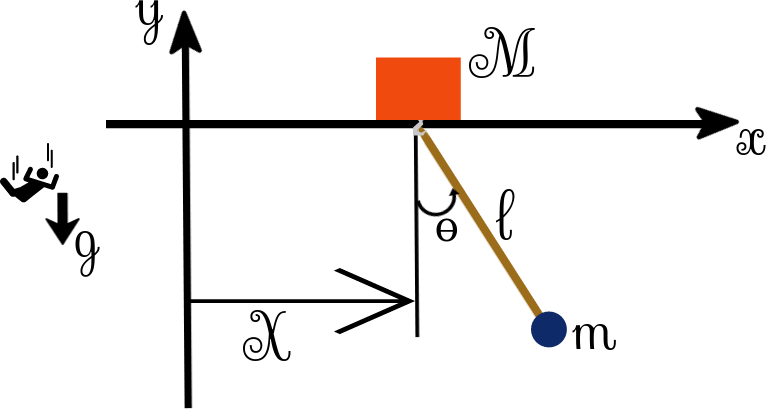
\includegraphics[scale=0.4]{problema3fig1}
 \caption{Representación gráfica del péndulo simple que tiene en su extremo fijo 
 una masa $M$ que puede moverse libremente en la dirección horizontal. Como indica 
 el muñequito la gravedad va dirigida hacia abajo.}
 \label{fig:problema3fig1}
\end{figure}

Tenemos entonces un péndulo simple cuyo extremo fijo está anclado a una masa $M$ que 
puede desplazarse libremente en dirección horizontal. Comencemos por ver cuantas coordenadas
generalizadas necesitamos para especificar la configuración del sistema completamente. 
Como trataremos este sistema como tridimensional, cada masa necesita tres coordenadas 
cartesianas para ser ubicada únicamente en el espacio, para $m$ las denotaremos por 
$(x,y,z)$ y para $M$, $(X,Y,Z)$. Pero debido a la configuración del sistema físico 
podemos ver fácilmente que existen cuatro constricciones holonómicas, que podemos 
escribir como\footnote{Es fácil ver que, debido al teorema de Pitágoras en coordenadas
cartesianas, $l$ se puede considerar como la hipotenusa de el triángulo formado 
por los catetos $y$ y $X-x$, y ya es claro el resultado de \mref{eq:pendu4}.}

\begin{align}
\label{eq:pendu1}
 Z &= 0, \\
\label{eq:pendu2}
 Y &= 0, \\
\label{eq:pendu3}
 z &= 0, \\
\label{eq:pendu4}
 [(x-X)^2 - y^2] - r^2 &= 0.
\end{align}

Las ecuaciones \mref{eq:pendu1, eq:pendu2} constriñen el movimiento de la masa $M$ 
al eje $X$. Las ecuaciones \mref{eq:pendu3, eq:pendu4} constriñen al péndulo a moverse 
en el plano $xy$ a lo largo de un arco de radio $l$, relativo a la masa movible $M$. Por 
lo tanto necesitamos $6-4 = 2$ coordenadas generalizadas para describir completamente 
la configuración del sistema. Las elecciones obvias para éstas son $X$, la cual denota 
la posición horizontal de la masa $M$, y $\theta$, que representa el desplazamiento 
angular del péndulo lejos del eje vertical.

\vspace{.3cm}

La formulación lagrangiana nos dice ahora que debeos obtener la energía cinética y la 
energía potencial en términos de las coordenadas generalizadas. Comenzamos por escribir 
la expresión de las mismas en coordenadas cartesianas, recordando que está presente un 
campo gravitacional constante dirigido hacia abajo,

\begin{align}
\label{eq:pendu5}
 T &= \frac{1}{2} M \dot{X}^2 + \frac{1}{2}m(\dot{x}^2+\dot{y}^2), \\
\label{eq:pendu6}
 V &= mgy
 \end{align}

Para poder expresar estas ecuaciones en términos de $X$ y $\theta$, necesitamos una 
transformación de coordenadas\footnote{Claramente la transformación de $X$ será $X = X$, 
y por lo tanto $\dot{X} = \dot{X}$.}, fáciles de obtener de la figura 
\mref{fig:problema3fig1},

\begin{align}
 x &= X + l \sen{\theta}, \\
 y &= -l \cos{\theta}
\end{align}

Ahora necesitamos la primera derivada temporal de las mismas para sustituirlas en 
la expresión de la energía cinética \mref{eq:pendu5},

\begin{align}
 \dot{x} &= \dot{X} + l \dot{\theta} \cos{\theta}, \\
 \dot{y} &= l \dot{\theta} \sen{\theta}
\end{align}

por lo tanto las ecuaciones \mref{eq:pendu5,eq:pendu6} se transforman en,

\begin{align}
 \begin{split}
  T &= \frac{1}{2} \dot{X}^2 + \frac{1}{2}m[(\dot{X}+ l \dot{\theta} \cos{\theta})^2 +
    (l \dot{\theta} \sen{\theta})^2], \\
    &= \frac{M}{2}\dot{X}^2 + \frac{m}{2}[\dot{X}^2 + 2l\dot{X}\dot{\theta}\cos{\theta} + 
    l^2 \dot{\theta}^2 \cos^2{\theta} + l^2 \dot{\theta}^2 \sen^2{\theta}], \\
    &= \frac{M}{2}\dot{X}^2 + \frac{m}{2}[\dot{X}^2 + l^2 \dot{\theta}^2 + 
    2l\dot{X}\dot{\theta}\cos{\theta}].
 \end{split}
\end{align}

\begin{equation}
 V = -mgl \cos{\theta}.
\end{equation}

Por lo tanto la lagrangiana $L = T - V$, será igual a 

\begin{equation}
 L = \frac{M}{2}\dot{X}^2 + \frac{m}{2}[\dot{X}^2 + l^2 \dot{\theta}^2 + 
    2l\dot{X}\dot{\theta}\cos{\theta}] + mgl \cos{\theta}.
\end{equation}

Y las ecuaciones de movimiento serán, para $X$,

\begin{equation}
 \frac{d}{dt}\frac{\partial L}{\partial \dot{X}} - \frac{\partial L}{\partial X} = 0,
\end{equation}

\begin{equation}
 \frac{d}{dt} (M \dot{X} + m \dot{X} + lm\dot{\theta}\cos{\theta}) = 0.
 \label{eq:pendu7}
\end{equation}

La ecuación \mref{eq:pendu7} es producto de que la lagrangiana no depende de $X$, y por 
lo tanto

\begin{equation}
 \boxed{M \dot{X} + m \dot{X} + l\dot{\theta}\cos{\theta} = \text{constante},}
\end{equation}

Lo cual nos dice que $M \dot{X} + m \dot{X} + lm\dot{\theta}\cos{\theta}$ es una integral 
de movimiento.

\vspace{.3cm}

Por otra parte para $\theta$,

\begin{equation}
  \frac{d}{dt}\frac{\partial L}{\partial \dot{\theta}} - \frac{\partial L}{\partial \theta} = 0,
\end{equation}

\begin{align}
\begin{split}
 \frac{d}{dt}(ml^2 \dot{\theta} + lm \dot{X} \cos{\theta}) + mgl\sen{\theta} +
 lm \dot{X} \dot{\theta} \sen{\theta} = 0, \\
 \ddot{m\theta}l^2  + m\ddot{X}l\cos{\theta} - \cancel{lm\dot{X}\dot{\theta}\sen{\theta}} + mgl\sen{\theta} +
 \cancel{lm \dot{X} \dot{\theta} \sen{\theta} = 0}. \\
 \end{split}
\end{align}

\begin{equation}
 \boxed{\therefore \ddot{\theta}  + \frac{\ddot{X}}{l}\cos{\theta} + \frac{g}{l}\sen{\theta} = 0.}
\end{equation}



\section{Problema 4}

Para un número de grados de libertad mayor que uno, dos lagrangianas distintas $L_1$
y $L_2$ generan ecuaciones de movimiento idénticas, demuestre que 

$$
L_1 - L_2 = \frac{d}{dt}f(q),
$$

donde $f$ es una función de la variedad de configuración en los reales. ¿Es esto cierto 
en sentido inverso?

\vspace{.3cm}

\underline{Solución:} \vspace{.3cm}

\textbf{Nota}: Debido a la alta aparición de sumatorias en este problema, durante la
solución del mismo utilizaremos el convenio de la suma de Einstein, el cual nos dice 
que un índice que aparece dos veces en un término matemático es sumado sobre 
el rango entero de ese índice.

\noindent\rule[0.5ex]{\linewidth}{1pt}

Comencemos por escribir las ecuaciones de Lagrange, donde $L = L(q^i,\dot{q}^i,t)$

\begin{equation}
 \frac{d}{dt}\frac{\partial L}{\partial \dot{q}^i} - \frac{\partial L}{\partial q^i} = 0 
\end{equation}

Por la regla de la cadena vemos que, 

\begin{align*}
 \xi_i (L) &\equiv \frac{\partial}{\partial \dot{q}^k}\frac{\partial L}{\partial \dot{q}^i} 
 \frac{d\dot{q}^k}{dt} + \frac{\partial}{\partial q^k}\frac{\partial L}{\partial \dot{q}^i} 
 \frac{dq^k}{dt} + \frac{\partial}{\partial t}\frac{\partial L}{\partial \dot{q}^i} \frac{dt}{dt}
 - \frac{\partial L}{\partial q^i}, \\
 &= \frac{\partial^2 L}{\partial \dot{q}^k\dot{q}^i} \ddot{q}^k + 
 \frac{\partial^2 L}{\partial q^k \dot{q}^i} \dot{q}^k+ \frac{\partial^2 L}{\partial t \partial \dot{q}^i}
 - \frac{\partial L}{\partial q^i}
 \end{align*}

Ahora, debido a que las lagrangianas producen las mismas ecuaciones de movimiento,
entonces 

\begin{align}
 \frac{\partial^2 L_1}{\partial \dot{q}^k\dot{q}^i} \ddot{q}^k + 
 \frac{\partial^2 L_1}{\partial q^k \dot{q}^i} \dot{q}^k+ \frac{\partial^2 L_1}{\partial t \partial \dot{q}^i}
 - \frac{\partial L_1}{\partial q^i} = \frac{\partial^2 L_2}{\partial \dot{q}^k\dot{q}^i} \ddot{q}^k + 
 \frac{\partial^2 L_2}{\partial q^k \dot{q}^i} \dot{q}^k+ \frac{\partial^2 L_2}{\partial t \partial \dot{q}^i}
 - \frac{\partial L_2}{\partial q^i}.
\end{align}

Que podemos escribir como,

\begin{equation}
 \xi_i (L_1) - \xi_i (L_2) = \frac{\partial^2 \phi}{\partial \dot{q}^k\dot{q}^i} \ddot{q}^k
 + \frac{\partial^2 \phi}{\partial q^k \dot{q}^i} \dot{q}^k + \frac{\partial^2 \phi}{\partial t \partial \dot{q}^i}  
 - \frac{\partial \phi}{\partial q^i} = 0.
 \label{eq:4cero}
 \end{equation}

Donde $\phi = L_1 - L_2$. Ahora, debido a que $L_1$ y $L_2$ son funciones de solamente 
$q^i,\dot{q}^i$ y $t$, entonces necesariamente $\phi$ también lo es, es decir, que 
$L_1$, $L_2$ y $\phi$ son lineales en $\ddot{q}^k$, por lo que

\begin{equation}
 \frac{\partial^2 \phi}{\partial \dot{q}^i\dot{q}^k} = 0,
 \label{eq:4phi0}
\end{equation}

y 

\begin{equation}
 \phi = \Xi_i (q,t) \dot{q}^i + \Gamma(q,t).
 \label{eq:4phi1}
\end{equation}

Y de \mref{eq:4phi1}, tenemos que 

\begin{equation}
 \frac{\partial \phi}{\partial \dot{q}^i} = \Xi_i,
 \label{eq:4xi1}
\end{equation}

y

\begin{equation}
 \frac{\partial \phi}{\partial q^i} = \frac{\Xi_k}{\partial q^i}\dot{q}^k + \frac{\Gamma}{\partial q^i}
\label{eq:4phipartial}
 \end{equation}


Entonces, tenemos que debido a \mref{eq:4phi0} la ecuación \mref{eq:4cero} se convierte en

\begin{equation}
 \frac{\partial^2 \phi}{\partial q^k \dot{q}^i} \dot{q}^k + \frac{\partial^2 \phi}{\partial t \partial \dot{q}^i}  
 - \frac{\partial \phi}{\partial q^i} = 0,
 \label{eq:4cero1}
\end{equation}

y sustituyendo \mref{eq:4xi1} y \mref{eq:4phipartial} en \mref{eq:4cero1} tenemos que

\begin{equation}
 \frac{\partial \Xi_i}{\partial q^k} \dot{q}^k + \frac{\partial \Xi_i}{\partial t}
- \frac{\Xi_k}{\partial q^i}\dot{q}^k - \frac{\Gamma}{\partial q^i} = 0,
\end{equation}

que podemos escribir como,

\begin{equation}
 \left( \frac{\partial \Xi_i}{\partial q^k} - \frac{\partial \Xi_i}{\partial q^i}\right) \dot{q}^k
 + \frac{\partial \Xi_i}{\partial t} - \frac{\Gamma}{\partial q^i} = 0.
\end{equation}

Pero debido a que las $Xi_i$ son lineales en $\dot{q}^k$, y usando un argumento 
parecido al que utilizamos anteriormente, vemos que 

\begin{equation}
 \frac{\partial \Xi_i}{\partial q^k} - \frac{\partial \Xi_i}{\partial q^i} = 0,
\end{equation}

\begin{equation}
 \therefore \frac{\partial \Xi_i}{\partial q^k} = \frac{\partial \Xi_i}{\partial q^i}.
\end{equation}

Y por lo tanto existe una función f(q,t) que nos permite escribir\footnote{Esto es una 
generalización para $n$ dimensiones del hecho de que en 3 dimensiones, $\nabla \times \mathbf{E} = 0$,
implica que existe una función $V$ tal que $\mathbf{E} = \nabla V$, que podemos escribir para 
$n$ dimensiones como $\partial E_i / \partial x_k = \partial E_k / \partial x_i$, 
$\therefore E_k = \partial V / \partial x_k$},

\begin{equation}
 \Xi_i = \frac{\partial f}{\partial q^i}
 \label{eq:4xi2}
\end{equation}

y por la ecuación anterior vemos que 

\begin{equation}
 \frac{\partial \Xi_i}{\partial t} = \frac{\partial \Gamma}{\partial q^i}
\end{equation}

\begin{equation}
 \frac{\partial}{\partial t}\frac{\partial f}{\partial q^i} = \frac{\partial \Gamma}{\partial q^i}
\end{equation}

\begin{equation}
 \therefore \Gamma = \frac{\partial f}{\partial t}
 \label{eq:4gamma}
\end{equation}

Ahora sustituyendo \mref{eq:4xi2} y \mref{eq:4gamma} en \mref{eq:4phi1} obtenemos que 

\begin{equation}
 \phi = \frac{\partial f}{\partial q^i}\dot{q}^i + \frac{\partial f}{\partial t}
\end{equation}

Pero por la regla de la cadena, y recordando que $\phi = L_1 - L_2$, tenemos que

\begin{equation}
 \boxed{L_1 - L_2 = \frac{d}{dt}f(q,t)}
\end{equation}

\vspace{.2cm} $\hspace{12cm} \square$

Entonces hemos demostrado la primera parte del problema. Ahora para la segunda parte 
de la demostración, podemos considerar el enunciado desde otra perspectiva. Lo que 
nos falta por demostrar es que si le sumamos a una lagrangiana una derivada total del tiempo
de una función como $f(q,t)$ entonces las ecuaciones de movimiento no cambiarán. Desde 
esta perspectiva podemos ver que si existe tal función $f(q,t)$ entonces,

\begin{equation}
 L' = L + \frac{df}{dt}
 \label{eq:4part1}
\end{equation}

también debe satisfacer las ecuaciones de Lagrange, hemos cambiado $L_1$ por $L'$ y 
$L_2$ por $L$, porque ya sabíamos que $L_1$ y $L_2$ satisfacen las ecuaciones de Lagrange, y
queremos hacer una demostración más general. Ahora podemos probar este resultado, asumiendo que 
$L$ satisface las ecuaciones de Lagrange. Derivemos \mref{eq:4part1} con respecto a $q^i$,

\begin{equation}
 \frac{\partial L'}{\partial q^i} = \frac{\partial L}{\partial q^i} + 
 \frac{\partial}{\partial q^i} \frac{df}{dt},
 \label{eq:4part2}
\end{equation}

y con respecto a $\dot{q}^i$,

\begin{equation}
 \frac{\partial L'}{\partial \dot{q}^i} = \frac{\partial L}{\partial \dot{q}^i} + 
 \frac{\partial}{\partial \dot{q}^i} \frac{df}{dt}.
 \label{eq:4part3}
\end{equation}

Podemos escribir para $f$ por la regla de la cadena,

\begin{equation}
 \frac{df}{dt} = \frac{\partial f}{\partial q^i}\dot{q}^i + \frac{\partial f}{\partial t}.
 \label{eq:4part4}
\end{equation}

Y entonces la derivada parcial de $df/dt$ con respecto a $\dot{q}^i$,

\begin{equation}
 \frac{\partial}{\partial \dot{q}^i} \frac{df}{dt} = \frac{\partial f}{\partial q^i}.
 \label{eq:4part5}
\end{equation}

Ahora tomando la derivada parcial de \mref{eq:4part3},

\begin{equation}
 \frac{d}{dt}\frac{\partial L'}{\partial \dot{q}^i} = \frac{d}{dt}\frac{\partial L}{\partial \dot{q}^i}
 + \frac{d}{dt}\frac{\partial f}{\partial q^i}.
 \label{eq:4part6}
\end{equation}

Ahora restando \mref{eq:4part6} menos \mref{eq:4part2}, 

\begin{equation}
 \frac{\partial L'}{\partial q^i} - \frac{d}{dt}\frac{\partial L'}{\partial \dot{q}^i} = 
 \frac{d}{dt}\frac{\partial L}{\partial \dot{q}^i}
 + \frac{d}{dt}\frac{\partial f}{\partial q^i} - \frac{\partial L}{\partial q^i} - 
 \frac{\partial}{\partial q^i} \frac{df}{dt}.
\end{equation}

Si arreglamos términos tenemos que 

\begin{equation}
  \frac{\partial L'}{\partial q^i} - \frac{d}{dt}\frac{\partial L'}{\partial \dot{q}^i} = 
\frac{d}{dt}\frac{\partial L}{\partial \dot{q}^i} - \frac{\partial L}{\partial q^i} + 
\frac{d}{dt}\frac{\partial f}{\partial q^i} - \frac{\partial}{\partial q^i} \frac{df}{dt}.
\label{eq:4part7}
\end{equation}

Pero por debido a que hemos asumido de entrada que  $L$ satisface las ecuaciones de 
Lagrange los primeros dos términos de \mref{eq:4part7} se hacen cero, y por otra parte 
que $f$ es diferenciable entonces,

\begin{equation}
 \frac{d}{dt}\frac{\partial f}{\partial q^i} =  \frac{\partial}{\partial q^i} \frac{df}{dt}.
\end{equation}

Y por lo tanto,

\begin{equation}
  \frac{\partial L'}{\partial q^i} - \frac{d}{dt}\frac{\partial L'}{\partial \dot{q}^i} = 0
\end{equation}

\vspace{.2cm} $\hspace{12cm} \square$

Hemos demostrado entonces que si existe una función de la forma $f(q,t)$, 
y al sumarle a una lagrangiana una derivada total temporal de ésta, entonces las 
ecuaciones de movimiento no se ven perturbadas, que era la otra parte de la demostración
que necesitábamos.

\section{Problema 5}

En presencia de la gravedad una partícula de masa $m$, inicialmente en reposo, se 
mueve a lo largo de una cicloide dada por 

$$
x = \pm a \cos^{-1}{\left(\frac{a-y}{a}\right)} + \sqrt{2ay-y^2}
$$

Encuentre y resuelva las ecuaciones de movimiento. Demuestre que el tiempo que tarda 
la partícula en llegar a la parte más baja del cicloide es independiente de su 
posición inicial sobre la cicloide.

\vspace{.3cm}

\underline{Solución:} \vspace{.3cm}

En la figura de abajo se encuentra el gráfico del cicloide en cuestión, de la ecuación 
vemos que este es válido para $y \in [0,2a]$ y en el eje $x$ lo graficamos de $[-\pi a, \pi a]$.

\begin{figure}[H]
 \center
 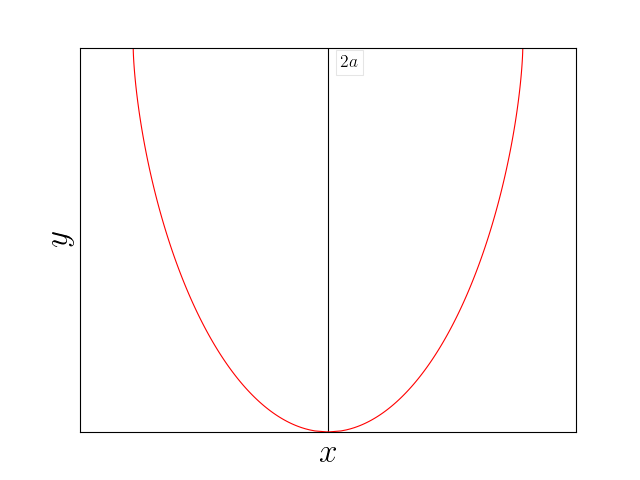
\includegraphics[scale=0.4]{problema5fig1}
 \caption{Gráfico del cicloide en consideración.}
 \label{fig:problema5fig1}
\end{figure}

Debido a las simetrías de este problema es claro que la coordenada generalizada que 
mejor describirá el sistema, en una manera más simple también, es la longitud de 
arco $s$ a lo largo de la línea definida por el cicloide (ver figura \mref{fig:problema5fig1}. 
En este caso, la energía cinética estará dada por 

\begin{equation}
 T = \frac{1}{2} m \dot{s}^2.
 \label{eq:energCinetCiclo1}
\end{equation}

Por otra parte, el potencial a la cual está sujeta la partícula, se puede obtener
simplemente de la fuerza de gravedad. Si imponemos que este campo gravitacional de 
magnitud $g$ está en la dirección negativa de $y$, entonces el potencial será,

\begin{equation}
 V = mgy.
 \label{eq:energPotenCiclo1}
\end{equation}

Debemos encontrar entonces la relación entre $y$ y $s$ para poder escribir la energía 
potencial en términos de nuestra coordenada generalizada. Recordando que la longitud 
de arco diferencial en coordenadas cartesianas se puede escribir como,

\begin{equation}
 s = \int \sqrt{dx^2+dy^2} = \int \sqrt{1+\left( \frac{dx}{dy} \right)^2} dy.
 \label{eq:arcoCartesiano}
\end{equation}

Ahora debemos obtener la derivada de $x$ con respecto a $y$, que hacemos explícitamente 
debajo,

\begin{align}
 \begin{split}
  %
  \frac{dx}{dy} &= \left(\pm a \cos^{-1}{\left(\frac{a-y}{a}\right)}\right)' + 
  \left(\sqrt{2ay-y^2}\right)', \\
  %
		&= a \left[ \frac{-1}{\sqrt{1 - \left(\frac{a-y}{a} \right)^2}}
		\left(\frac{a-y}{a} \right)'\right] + \frac{1}{2\sqrt{2ay-y^2}}
		(2ay - y^2)', \\
  %
		&= \cancel{a}\left[ \frac{-1}{\sqrt{1 - \left(\frac{a-y}{a} \right)^2}}
		\left(- \frac{1}{\cancel{a}} \right) \right] + \frac{1}{\cancel{2}\sqrt{2ay-y^2}}
		[\cancel{2}(a - y)], \\
  %
		&= \frac{1}{\sqrt{1 - \frac{(a-y)^2}{a^2}}} + \frac{a-y}{\sqrt{2ay - y^2}}.
  %
 \end{split}
\end{align}

Y simplificando llegamos a que 

\begin{equation}
 \frac{dx}{dy} = \frac{2a - y}{\sqrt{2ay - y^2}}
 \label{eq:dxdyCiclo}
\end{equation}

Ahora sustituyendo \mref{eq:dxdyCiclo} en \mref{eq:arcoCartesiano} nos queda 

\begin{equation}
 s = \int \sqrt{1 + \frac{(2a - y)^2}{(\sqrt{2ay - y^2})^2}} dy,
\end{equation}

que podemos reescribir como

\begin{align}
\begin{split}
 %
 s &= \int \sqrt{1 + \frac{(2a - y)^2}{2ay - y^2}} dy, \\
 % 
   &= \int \sqrt{\frac{2ay - \cancel{ y^2} + 4a^2 - 4ay + \cancel{y^2}}{2ay - y^2}} dy, \\  
 % 
   &= \int \sqrt{\frac{4a^2 -2ay}{2ay - y^2}} dy.  \\
 %
   &= \int \sqrt{2} \sqrt{\frac{a}{y}} dy.
 \end{split}
\end{align}

Evaluando esta integral obtenemos que 

\begin{equation}
 s = 2 \sqrt{2ay}.
\end{equation}

Y por lo tanto

\begin{equation}
 y = \frac{s^2}{8a}.
 \label{eq:yCiclo}
\end{equation}

Sustituyendo \mref{eq:yCiclo} en \mref{eq:energPotenCiclo1}, obtenemos 

\begin{equation}
 V = \frac{mgs^2}{8a}
\end{equation}

Entonces la lagrangiana del sistema, $L = T - V$ es 

\begin{equation}
 L = \frac{1}{2} m \dot{s}^2 - \frac{mgs^2}{8a}
\end{equation}

Y utilizando las ecuaciones de Lagrange\footnote{Tomando en cuenta que el sistema es conservativo.} 


\begin{equation}
 \frac{d}{dt}\frac{\partial L}{\partial \dot{s}} - \frac{\partial L}{\partial s} = 0,
\end{equation}

tenemos que la ecuación de movimiento del sistema será:

\begin{equation}
 \frac{d}{dt} (m\dot{s}) - \frac{mgs}{4a} = 0,
\end{equation}

\begin{equation}
 \boxed{\therefore \ddot{s} = \frac{g}{4a} s.}
\end{equation}

Claramente esta es la ecuación de un oscilador armónico, y podemos ver esto de una 
forma un poco más clara si llamamos $k = g/4a$, entonces la ecuación de movimiento 
se convierte en

\begin{equation}
 \ddot{s} - ks = 0.
\end{equation}

Cuya solución es\footnote{Esta solución ya se ha encontrado en otras tareas 
varias veces, y es muy simple obtenerla. Debido a que es una ecuación diferencial lineal
de segundo orden homogénea proponemos una solución del tipo $\euler^{\lambda t}$, obtenemos la 
ecuación característica de la EDO. Luego obtenemos las raíces $\lambda$ que sustituiremos
en la solución que hemos propuesto, haciendo uso de la linealidad de la ecuación para 
usar el principio de superposición y sumar estas soluciones. Por último hacemos la 
sustitución $A = \sqrt{C_1^2+ C_2^2}$, donde $C_1$ y $C_2$ son las constantes de 
integración de la ecuación diferencial, y con un poco de trigonometría, colocamos 
$C_1$ y $C_2$ en un triángulo rectángulo de hipotenusa $A$, y proponemos un ángulo
$\delta$ entre $A$ y $C_1$, al cual llamamos fase de la oscilación.},

\begin{equation}
 s = A\cos{(\omega t + \delta)}
\end{equation}

donde $\omega = \frac{1}{2}\sqrt{g/a}$ es la frecuencia del oscilador, $A$ es la 
amplitud de la oscilación y $\delta$ es la fase de la misma. La cual es la solución
clásica para un oscilador armónico en $s$.

\vspace{.3cm}

La demostración de que el tiempo que tarda la partícula en llegar a la parte más baja 
del cicloide es independiente de su posición inicial sobre la cicloide, es ahora 
trivial debido a que tenemos un oscilador armónico y entonces, con un poco de ayuda 
de la figura \mref{fig:problema5fig1} y usando los resultados de la teoría de 
osciladores armónicos, es fácil ver que el tiempo que le tomará a la partícula 
llegar a la parte más baja del cicloide es un cuarto de período, independientemente de 
la amplitud (que es lo mismo que considerar su posición inicial en el cicloide).


\end{document}

